\documentclass{article}
\usepackage{../HBSuerDemir}
\begin{document}
\hPage{b2p2/412} 


When S is given by (1') (or by 1"), d$\sigma$ can be projected to one of the coordinate 
 planes in which the transformed double integral is simpler. If S is projected onto
 xy-plane, say, (1') becomes 
  \begin{itemize}
 \item[] $\iint_S P cos(\alpha) + 0  cos(\beta) + R cos(\gamma)) sec(\gamma) dxdy$
  \end{itemize}
 \begin{itemize}
	\item[] Example 1. Evaluate 
	where S is the surface $x = y^2 + z^2,    0 \leq x \leq 4$ 
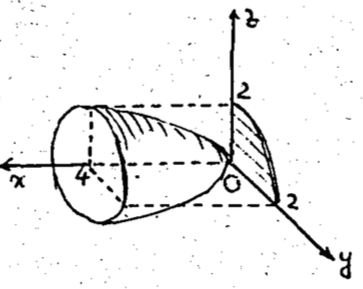
\includegraphics[width = 0.65\textwidth,height = 0.25\textheight]{images/graph3} \\
 Solution. R(yz) : $y^2 + z^2 = 4$
 \begin {equation}
 $$ \[ \int_2^2 \! \int_{-\sqrt{4-y^2}}^{\sqrt{4-y^2}} y^2+z^2-z\,dz\,dy.\] $$
 $$\[ \int_2^2 \! y^2 z + \frac{z^3}{3} - \frac{z^2}{2}\Big|_{-\sqrt{4-y^2}}^{\sqrt{4-y^2}} dy\]$$
$$ \[2\int_{-2}^{2 }y^2 \sqrt{4-y^2}+\frac{1}{3} (4-y^2) \sqrt{4-y^2}  dy\] $$
 $$\[2\int_{-2}^{2 }frac{2}{3}y^2 \sqrt{4-y^2}+\frac{4}{3} \sqrt{4-y^2}  dy\] $$
 $$\[= \frac{8}{3} \pi +\frac{16}{3} \pi = 8\pi \]$$
\end {equation}
 	\item[] Example 2.Evaluate
 \end{itemize}
  \begin {equation}
 $$\[I = \iint_S x^2< \,dy\,dz + y^2x dzdx  + xy dxdy\]$$
  \end {equation}
 
 where S is the cone $x^2 + y^2 = (z-4)^2 $  with $0 \leq z \leq 4$
 
 
\end{document}
